% Auto-generated from docs/schematic/spec_bio.py via render.py — edit the template, not the .tex.
\documentclass[tikz,border=6pt]{standalone}
\usepackage{amsmath}
\usepackage{tikz}
\usetikzlibrary{arrows.meta,calc}
\definecolor{predcolor}{HTML}{4C8DFF}
\definecolor{errcolor}{HTML}{E0772B}
\definecolor{regionstroke}{HTML}{222222}
\definecolor{relaystroke}{HTML}{888888}
\definecolor{interfill}{HTML}{6E6E6E}
\definecolor{rulecol}{HTML}{C9C9C9}
\definecolor{titlecol}{HTML}{222222}
\begin{document}
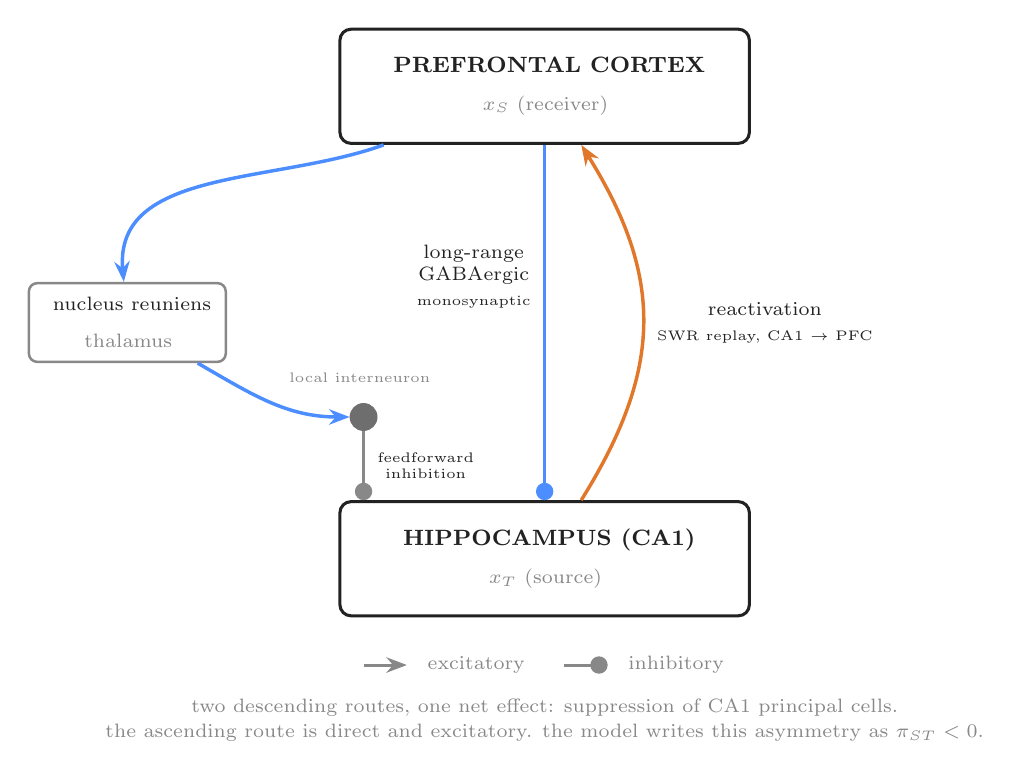
\begin{tikzpicture}[
  % --- nodes ---
  region/.style={rounded corners=4pt, draw=regionstroke, line width=1.1pt, fill=white,
                 align=center, inner sep=3pt, text=titlecol},
  relay/.style={rounded corners=3pt, draw=relaystroke, line width=0.9pt, fill=white,
                align=center, inner sep=3pt, text=titlecol},
  inter/.style={circle, draw=interfill, fill=interfill, minimum size=3.4mm, inner sep=0pt},
  value/.style={circle, draw=regionstroke, line width=1.1pt, fill=white,
                align=center, inner sep=0pt, text=titlecol},
  err/.style={rounded corners=3pt, draw=relaystroke, dashed, line width=0.9pt, fill=white,
              align=center, inner sep=2pt, text=titlecol},
  ghost/.style={inner sep=0pt, minimum size=0pt},
  % --- couplings: colour = direction, terminal = sign ---
  down/.style={predcolor, line width=1.25pt},
  up/.style={errcolor, line width=1.25pt},
  local/.style={relaystroke, line width=1.1pt},
  corr/.style={relaystroke!75, line width=0.7pt, dotted},
  excit/.style={-{Stealth[length=2.6mm]}},
  inhib/.style={-{Circle[length=2.2mm, width=2.2mm]}},
  selfloop/.style={-{Stealth[length=2.2mm]}, relaystroke, line width=0.9pt, looseness=11},
  % --- lettering ---
  glab/.style={font=\scriptsize, fill=white, inner sep=1.5pt, align=center, text=titlecol},
  note/.style={font=\scriptsize, text=relaystroke, align=center},
  panel/.style={font=\scriptsize\bfseries, text=relaystroke, align=center},
  lgd/.style={font=\scriptsize, text=relaystroke},
]
% ---- regions, relays, interneurons ----
\node[region, minimum width=5.20cm, minimum height=1.45cm] (pfc) at (0.00,-0.00) { { \footnotesize\bfseries PREFRONTAL CORTEX }\\[1.5pt]{ \scriptsize\color{relaystroke} $x_S$ (receiver) } };
\node[region, minimum width=5.20cm, minimum height=1.45cm] (hpc) at (0.00,-6.00) { { \footnotesize\bfseries HIPPOCAMPUS (CA1) }\\[1.5pt]{ \scriptsize\color{relaystroke} $x_T$ (source) } };
\node[relay, minimum width=2.50cm, minimum height=1.00cm] (re) at (-5.30,-3.00) { { \scriptsize nucleus reuniens }\\[1.5pt]{ \scriptsize\color{relaystroke} thalamus } };
\node[inter] (inn) at (-2.30,-4.20) {  };

% ---- recurrent self-loops ----

% ---- projections ----
\draw[down, inhib] (pfc) to[out=-90, in=90] node[glab, pos=0.36, anchor=east, xshift=-3pt]{ long-range\\GABAergic\\[1pt]{\tiny monosynaptic} } (hpc);
\draw[down, excit] (pfc) to[out=200, in=95] (re);
\draw[down, excit] (re) to[out=-30, in=180] (inn);
\draw[local, inhib] (inn) to[out=-90, in=90] node[glab, pos=0.5, anchor=west, xshift=3pt, font=\tiny]{ feedforward\\inhibition } (hpc.north -| inn);
\draw[up, excit] (hpc) to[out=58, in=-58, looseness=1.12] node[glab, pos=0.5, anchor=west, xshift=3pt]{ reactivation\\[1pt]{\tiny SWR replay, CA1 $\to$ PFC} } (pfc);

% ---- panel rules ----

% ---- captions ----
\node[note, anchor=center] at (-2.30,-3.70) { {\tiny local interneuron} };
\node[note, anchor=center] at (0.00,-8.05) { two descending routes, one net effect: suppression of CA1 principal cells.\\[1pt]the ascending route is direct and excitatory. the model writes this asymmetry as $\pi_{ST}<0$. };

% ---- legend: arrowhead = excitatory, dot = inhibitory ----
\draw[local, excit, line width=1.1pt] (-2.30,-7.35) -- ++(0.55,0);
\node[lgd, anchor=west] at (-1.61,-7.35) { excitatory };
\draw[local, inhib, line width=1.1pt] (0.25,-7.35) -- ++(0.55,0);
\node[lgd, anchor=west] at (0.94,-7.35) { inhibitory };

\end{tikzpicture}
\end{document}